% Dossier de qualité
% Version 1.2

% Historique des versions
% 19/01/08 1.0 Création et remplissage (Mikado)
% 20/01/08 1.1 Mise en page un peu plus jolie (Mikado)
% 31/01/08 1.2 Mise à jour pour évolution du contenu : ajout du PAQP

\documentclass[a4paper, 11pt, draft]{report}

\usepackage[frenchb]{babel}
\usepackage[utf8]{inputenc}
\usepackage{aeguill}
\usepackage[final]{graphicx}
\usepackage{geometry}
\usepackage{fancyhdr}
\usepackage{url}
\usepackage[pdftex, hypertexnames=false, colorlinks=true, final]{hyperref}
\usepackage[Lenny]{fncychap}

% Marges à gauche et à droite de 3cm
\geometry{margin=3cm}

% Utilisation des headers et footers personnalisés de fancyhdr
\pagestyle{fancy}

% Images dans le dossier ./images/
\graphicspath{{./images/}}

% Gestion des métadonnées étranges à rendre visibles au rendu
\newcommand\docname{DQv1.2}
\newcommand\docauthor{Fabrice GABOLDE}
\newcommand\docstatus{LIVRABLE}

% Format de citation de références standard, marche avec quasiment tout
\newcommand\fullref[1]{\ref{#1}, page \pageref{#1}}

% Numérotation : part remet à zéro les chapitres (parce que je veux)
\makeatletter\@addtoreset{chapter}{part}\makeatother

% En-têtes et pieds de page
\lhead{\docname}
\rhead{}
\lfoot{Auteur : H4213}
\cfoot{}
\rfoot{\thepage}

% Titre du document maître
\title{\textbf{COPEVUE}\\
\rule{\textwidth}{1pt}{}\\
\Huge{\textsc{Dossier de qualité}}}
\author{\docauthor{} (H4213)}
\date{\docname{} --- \today{} (\docstatus{})}

\begin{document}

\maketitle

\tableofcontents

% Dossier de gestion de la documentation
% Version 1.2

% Historique des versions
% 19/01/08 1.0 Création et remplissage (Mikado)
% 20/01/08 1.1 Entrée en phase de finalisation (Mikado)
% 21/01/08 1.2 Finalisation du document (Mikado)

\renewcommand\docname{DGDv1.2}
\renewcommand\docauthor{Fabrice GABOLDE}
\renewcommand\docstatus{LIVRABLE}
\part{Dossier de gestion de la documentation}

\label{part:dgd}

\chapter{Introduction}

\section*{Document \docname{}}

Auteur : \docauthor{}

Etat : \docstatus{}

\section{Présentation du projet}

Il existe aujourd'hui de nombreux sites isolés et/ou difficiles d'accès qui nécessitent une surveillance et parfois des actions à distance. Ces sites se situent dans des espaces très différents tels que les citernes placées dans les forêts escarpées du pourtour méditerranéen, les réservoirs utilisés pour l'autonomie des chantiers dans le grand Nord mais aussi les personnes âgées qui se retrouvent souvent isolées.

Actuellement tous les contrôles et actions sont réalisés par un opérateur qui doit se déplacer sur le site. Il n'y a donc que très peu de réactivité, on ne peut pas avoir un suivi fin des évolutions et des problèmes graves (par exemple la fuite d'un réservoir) ne peuvent pas être traités rapidement.

\paragraph{Etude COPEVUE}
L'objet de l'étude est la mise en place d'un système générique de surveillance et d'action à distance sur des sites isolés. Le système devra être évolutif, autonome et fiable.

\section{Présentation du document}

Ce document (Dossier de gestion de la documentation) présente les différentes normes et suggestions applicables à la production de documents dans le cadre du projet COPEVUE. Le but de ce document est de fournir une base pour assurer la qualité du projet dans son ensemble.

\subsection{Objectifs}

Voici les objectifs de ce document :
\begin{itemize}
\item Présentation des documents à produire
\item Présentation des règles de production
\item Définition du cycle de vie, états et version d'un document
\item Présentation de la gestion des documents produits
\item Présentation de la gestion des fichiers et dossiers
\item Présentation de la gestion de la communication interne
\end{itemize}

\section{Documents applicables et de référence}

\subsection{Documents applicables}

\begin{itemize}
\item Dossier de gestion de la documentation (DGD), ce document
\end{itemize}

\subsection{Documents de référence}

Aucun.

\chapter{Règles générales}

\section{Identification des documents}

Les documents seront identifiés par une abréviation standard et leur numéro de version (exem\-ple pour ce dossier de gestion de la documentation : \docname). Le numéro de version sera incrémenté à chaque contribution au document.

\section{Norme de présentation}

Les documents présenteront le même style et la même page de garde (aux informations propres à chaque document près : titre, version, etc.) dans un but d'uniformisation.
Voir \fullref{chapter:modeles_documents} pour les modèles de documents utilisés.

\section{Etats d'un document}

Un document doit à tout moment être parmi l'un de ces états (voir figure \fullref{figure:dossier_gestion_documentation_etats_documents}) :
\begin{description}
\item[En cours]{Le document est en cours de rédaction par son (ou ses) auteur(s), et n'est pas encore présentable ni même vérifié. L'option \verb|draft| doit être présente dans les options globales du document.}
\item[Attente]{Le document est en attente de vérification par le CdP, sa rédaction est arrêtée ; il peut repasser \textbf{en cours} si le CdP a des remarques à faire concernant le contenu. L'option \verb|draft| doit être présente dans les options globales du document.}
\item[Validé]{Le document a été validé pour son contenu par le CdP ; il peut repasser \textbf{en cours} si le RQ a des remarques à faire concernant la conformité. L'option \verb|draft| doit être présente dans les options globales du document.}
\item[Livrable]{Le document a été validé pour sa conformité par le RQ. L'option \verb|draft| doit être remplacée dans les options globales du document par l'option \verb|final|.}
\end{description}

\begin{figure}[!htp]
\begin{center}
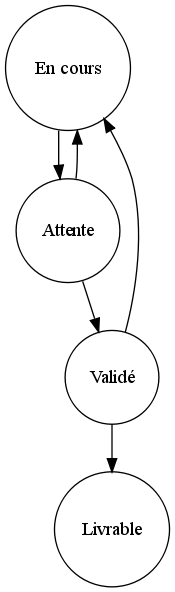
\includegraphics[width=0.15\textwidth]{qualite_dossier_gestion_documentation_etats_documents.png}
\caption{Etats d'un document}
\label{figure:dossier_gestion_documentation_etats_documents}
\end{center}
\end{figure}

\section{Cycle de vie d'un document}

\subsection{Production du document}

L'auteur principal du document est le collaborateur, ou le groupe de collaborateur, désigné par le CdP pour travailler dessus en priorité. Les autres membres du groupe de travail peuvent ensuite participer à la production du document si nécessaire. L'auteur principal doit commencer la production du document en mettant en place le template \LaTeX{} fourni pour ce type de document et le plan général du document. Il peut pour ce faire s'aider des plans types (voir \fullref{chapter:plans_types}).

\subsection{Vérification et validation du document}

La vérification du document se fait en deux étapes : d'abord, le CdP vérifie le contenu du document. Il peut à ce stade le renvoyer à l'auteur principal si des problèmes ont été relevés. Puis, le RQ vérifie la conformité du document. De même, il peut à ce stade le renvoyer à l'auteur principal en cas de non-conformité trop importante.

\subsection{Archivage du document}

L'archivage du document est géré par le système de contrôle de version employé. A tout moment, sur le serveur SVN maintenu par le groupe de travail, on peut retrouver la dernière version de tout document produit, ou l'une des versions précédentes.

\section{Gestion des versions}

La numérotation des versions se fait en \verb|major.minor| et suit les règles suivantes :
\begin{itemize}
\item A la création, le numéro de version est 1.0
\item Chaque modification non-triviale (exemple de modification triviale : correction d'une ou deux fautes d'orthographe) entraîne une incrémentation du numéro mineur de version
\item Chaque modification de grande envergure (exemple de modification de grande envergure : modification du plan, changement radical du contenu \ldots) entraîne une incrémentation du numéro majeur de version et une remise à zéro du numéro mineur de version
\end{itemize}

\chapter{Gestion de la documentation produite}

\section{Documents applicables et de référence}

\subsection{Documents applicables}

Un document applicable contient des indications qui doivent être suivies à la lettre pour assurer la qualité de la production des documents qui le référencent. Un document qui référence un document applicable, mais ne le respecte pas, n'est pas validable par le responsable qualité. Par exemple :
\begin{itemize}
\item Modèle de document livrable
\item Modèle de revue de document par le responsable qualité
\item \ldots
\end{itemize}

\subsection{Documents de référence}

Un document de référence contient des indications qui n'ont pas besoin d'être suivies à la lettre, mais qui peuvent aider à la production des documents qui le référencent. Un document qui référence un document de référence, mais qui ne le respecte pas, peut tout de même être validable par le responsable qualité. Les plans types (voir \fullref{chapter:plans_types}) entrent dans la catégorie des documents de référence.

\section{Gestion physique des fichiers contenant les documents}

\subsection{Répertoires}

Chaque document produit sera placé dans son propre répertoire. Le nom du répertoire utilisé sera celui de l'abréviation du document (voir le glossaire pour les abréviations), par exemple DGD pour le dossier de gestion de la documentation. Les dossiers relatifs à la qualité seront de plus situés dans le répertoire \url{qualite/}, et ceux relatifs au travail du CdP dans le répertoire \url{cdp/}. Les images utilisées pour chaque document seront dans leur propre sous-répertoire \url{images/}, par exemple pour les images du DGD : \url{qualite/dgd/images/}.

\subsection{Procédures de sauvegarde et archivage}

Les procédures de sauvegarde et d'archivage sont celles permises par l'utilisation normale du système de contrôle de version SVN.

\chapter{Communication interne}

Le groupe de travail utilisera un certain nombre de moyens de communication en interne :
\begin{description}
\item[Réunions IRL]{Des réunions en personne auront lieu tant pendant les horaires de TP prévus par le programme qu'en dehors, en fonction des nécessités des collaborateurs et du planning du CdP.}
\item[e-mail]{Tous les membres du groupe de travail disposent d'une adresse e-mail qui a été communiquée au reste du groupe au début du projet. L'envoi d'e-mails peut servir, d'une part entre collaborateurs pour s'échanger de grandes quantités de données qui n'auraient pas lieu d'être présentes sur le serveur SVN, d'autre part au CdP pour coordonner son équipe.}
\item[IM]{Tous les membres du groupe de travail disposent d'une adresse liée à un protocole de messagerie instantanée pour assurer la communication à distance via Internet, tant en temps réel qu'en asynchrone.}
\item[SVN]{L'utilisation de SVN permet de laisser des commentaires à chaque remontée de contenu, et donc d'informer le reste de l'équipe sur ce qui a été modifié.}
\end{description}
% PAQP
% Version 1.1

% Historique des versions
% 27/01/08 1.0 Création et remplissage (Mikado)
% 30/01/08 1.1 Fin du draft (Mikado)

\renewcommand\docname{PAQPv1.1 (DRAFT)}
\renewcommand\docauthor{Fabrice GABOLDE}
\renewcommand\docstatus{EN COURS (DRAFT)}
\part{Plan d'assurance qualité projet}

\chapter{Introduction}

\section*{Document \docname{}}

Auteur : \docauthor{}

Etat : \docstatus{}

\section{Présentation du projet}

Il existe aujourd'hui de nombreux sites isolés et/ou difficiles d'accès qui nécessitent une surveillance et parfois des actions à distance. Ces sites se situent dans des espaces très différents tels que les citernes placées dans les forêts escarpées du pourtour méditerranéen, les réservoirs utilisés pour l'autonomie des chantiers dans le grand Nord mais aussi les personnes âgées qui se retrouvent souvent isolées.

Actuellement tous les contrôles et actions sont réalisés par un opérateur qui doit se déplacer sur le site. Il n'y a donc que très peu de réactivité, on ne peut pas avoir un suivi fin des évolutions et des problèmes graves (par exemple la fuite d'un réservoir) ne peuvent pas être traités rapidement.

\paragraph{Etude COPEVUE}
L'objet de l'étude est la mise en place d'un système générique de surveillance et d'action à distance sur des sites isolés. Le système devra être évolutif, autonome et fiable.

\section{Présentation du document}

Ce document (Plan d'assurance qualité projet) couvre toute la conception du système d'un point de vue qualité, jusqu'à la réception par le client.

\subsection{Objectifs}

Voici les objectifs de ce document :
\begin{itemize}
\item Présenter l'organisation humaine du comité de pilotage
\item Présenter la démarche de qualité au niveau du processus
\item Rappeler les règles de documentation
\item Présenter la gestion de la configuration
\item Présenter les outils et méthodes à utiliser
\item Proposer une méthode de suivi de l'application du Plan Qualité
\end{itemize}

\section{Documents applicables et de référence}

\subsection{Documents applicables}

\begin{itemize}
\item Dossier de gestion de la documentation (DGD)
\end{itemize}

\subsection{Documents de référence}

Aucun.

\chapter{Organisation humaine du comité de pilotage du projet}

\section{Rôle des différents intervenants}

\subsection{Maîtrise d'\oe uvre : Chef de projet}

Le chef de projet anime l'équipe et les séances de travail. Il a une vue d'ensemble du projet et de ces objectifs et il planifie le déroulement de l'étude.

\subsection{Maîtrise d'\oe uvre : Responsable Qualité}

Le responsable qualité épaule le chef de projet dans son travail en définissant l'environnement de qualité dans lequel le projet doit se dérouler.

\subsection{Maîtrise d'\oe uvre : Groupe d'Études en Informatique}

Les experts du GEI sont chargés de l'étude technique du projet.

\section{Relations entre les intervenants}

\begin{figure}[!htp]
\begin{center}
\includegraphics[width=0.45\textwidth]{qualite_paqp_relations_intervenants_moe.png}
\caption{Relations entre les intervenants}
\label{figure:paqp_relations_intervenants}
\end{center}
\end{figure}

\chapter{Qualité au niveau du processus}

\section{Présentation de la démarche de développement au niveau Projet}

Cycle de développement :
\begin{itemize}
\item Etude préalable
\item Etude détaillée
\item Etude technique
\item Réalisation
\item Mise en \oe uvre.
\end{itemize}

\section{Règles de qualité pour l'ingénierie concurrente}

Utilisation des normes par ordre croissant de priorité :
\label{list:normes}
\begin{itemize}
\item Langage (guides de style propres aux langages utilisés)
\item Outils de développement (suivi des normes imposées ou admises pour le processus de développement usuel avec les outils utilisés)
\item Formalismes utilisés par la méthode de développement suivie
\item Normes générales COPEVUE
\end{itemize}

Utilisation des techniques habituelles de développement concurrent (éditeurs collaboratifs ou systèmes de suivi de versions, etc.).

Respect des normes de la gestion de documentation : voir le chapitre \fullref{chapter:documentation} et le DGD en partie \fullref{part:dgd}.

Respect des procédures de gestion des modifications (chapitre \fullref{chapter:mods}), et d'un point de vue général, des normes habituellement utilisées par COPEVUE.

\chapter{Documentation}

\label{chapter:documentation}

Voir le DGD, partie \fullref{part:dgd}, pour le détail des règles utilisées pour la gestion de la documentation.

\chapter{Gestion de configuration}

\section{Découpage en éléments de configuration logicielle}

On se réfèrera pour cette partie à l'ensemble des cahiers des charges (voir les documents correspondants). Utilisation de modules indépendants mais intercommunicants : API unifiée.

\section{Conventions d'identification}

\section{Procédures d'identification des éléments de configuration}

\section{Gestion des ressources partagées}

Adoption du même système que pour l'élaboration des dossiers précédents : système de gestion de versions (SVN), accès à distance au serveur commun (SSH), etc.

\chapter{Gestion des modifications}

\label{chapter:mods}

\section{Origines des modifications}

Traiter en particulier les modifications provenant du client, puis celles provenant des autres services de COPEVUE et les requêtes des éventuels sous-traitants.

\section{Procédures et organisation des modifications}

Pour les modifications émanant du client : étudier la faisabilité tant que le projet n'a pas dépassé un certain degré d'avancement, les mettre en place si possible, faire remonter l'information à tous les services concernés ; si trop tard ou modifie trop de volume de développement, refuser la modification (les dossiers techniques ayant déjà été validés).

\chapter{Méthodes et outils}

\section{Méthodes}

Méthodes usuelles du développement concurrent en ingénierie. UML, etc.

\section{Outils}

\section{Normes}

Voir la liste en section \fullref{list:normes}.

\chapter{Contrôle des fournisseurs}

\section{Exigences vis à vis des sous-traitants}

Contrat qualité défini grâce à la charte qualité de COPEVUE et aux engagements des sous-traitants.

\section{Logiciels achetés, loués ou imposés}

\chapter{Copie, protection et livraison}

\section{Précautions à prendre lors de la copie}

Assurer une qualité maximale et une perte de données minimales lors de la copie. Ne fournir à l'extérieur que des copies zéro-défaut : calcul de hachages pour comparer à une copie maître.

\section{Précautions relatives au stockage des logiciels}

Attention au stockage sur médium externe (CD, etc.) : corruption des matériaux. Stockage sur serveurs : doublons (éviter pertes de données), mais protégés, avec si possible une copie offline (éviter fuites\ldots).

\section{Modalités de livraison}

\chapter{Suivi de l'application du Plan Qualité}

\section{Responsabilités}

\section{Techniques de vérification}

\begin{itemize}
\item Evidemment, auto-contrôle, relecture, etc.
\item Lectures croisées
\item Inspections
\item Revues, audits ?
\item Qualimétrie précise
\end{itemize}
% Annexes au dossier de qualité
% Version 1.2

% Historique des versions
% 20/01/08 1.0 Création et remplissage (Mikado)
% 21/01/08 1.1 Plans types : STB et DCNS (Mikado)
% 23/01/08 1.2 Plan type : CDC (Mikado)

% \renewcommand\thechapter{\alph{chapter}}
\renewcommand\docname{ANNEXESv1.1}
\appendix

\chapter{Modèles de documents}

\label{chapter:modeles_documents}

L'uniformisation des documents est obtenue en utilisant des templates \LaTeX{} définis par le responsable qualité, en accord avec le reste du groupe.

\section{Modèle de document livrable}

\paragraph{}
Un document livrable doit présenter les informations suivantes :
\begin{itemize}
\item En page de garde :
\begin{itemize}
\item Le titre du projet
\item Le titre du document
\item L'auteur principal du document
\item L'auteur (hexanôme) du document
\item L'identification du document
\item La date de compilation telle qu'obtenue par la commande \verb|\today|
\item L'état du document
\end{itemize}
\item En en-tête :
\begin{itemize}
\item L'identification du document courant
\end{itemize}
\item En bas de page :
\begin{itemize}
\item L'auteur (hexanôme) du document
\item Le numéro de la page courante dans le document
\end{itemize}
\end{itemize}
Certaines informations ne seront accessibles que via la lecture de la source du document, par exemple l'historique des versions (qui permet d'obtenir la dernière personne à avoir contribué au document, sa contribution, les dates de création et de modification\ldots).

Il faut également noter que pour respecter au maximum les règles de la bonne typographie, certaines pages (nouveaux chapitres) ne présentent pas toutes les informations dans les en-têtes et pieds de page.

\paragraph{}
Un document livrable doit commencer par le chapitre d'introduction, qui comporte les sections suivantes : 

(Dans le corps de l'introduction : identification, auteur et état du document)
\begin{enumerate}
\item Présentation du projet
\item Présentation du document
\begin{enumerate}
\item Objectifs
\end{enumerate}
\item{Documents applicables et de référence}
\begin{enumerate}
\item Documents applicables
\item Documents de référence
\end{enumerate}
\end{enumerate}

\chapter{Plans types}

\label{chapter:plans_types}

\section[STB]{Dossier de spécification technique des besoins}

\begin{enumerate}
\item{Introduction}
\item{Axes d'amélioration retenus}
\begin{enumerate}
\item{Axes de progrès retenus}
\item{Axes de progrès marginaux}
\item{Faux axes de progrès éventuels}
\end{enumerate}
\item{Description des exigences fonctionnelles du futur système}
\item{Description des exigences non fonctionnelles du futur système}
\item{Impacts de la nouvelle solution sur le système}
\item{Bilan des améliorations}
\item{Conclusion}
\end{enumerate}

\section[CNS]{Dossier de conception de nouveau système}

\begin{enumerate}
\item Introduction
\item Organisation générale de l'atelier
\item Règles de pilotage de l'atelier
\item Architecture applicative
\item Architecture informatique et matérielle
\item Réflexions sur les données
\item Gestion des anomalies et sécurité
\item Conclusion
\item[A]{Annexe : Représentation informatique des objets technologiques}
\item[B]{Annexe : Réflexion sur le réseau}
\item[C]{Annexe : Démarrage du système}
\end{enumerate}

\section[CDC]{Cahier des charges}

\begin{enumerate}
\item Introduction
\item Objectif du logiciel
\item Exigences fonctionnelles
\item Contraintes imposées et faisabilité technologique
\item Configuration cible
\item[A]{Annexe : Etude préalable}
\item[B]{Annexe : Etude de faisabilité}
\end{enumerate}


\end{document}